% Source: 1959 全国 第4题解答，原PDF第5页，解答末图。
% AB=BC=a, ∠APB=90°, ∠BPC=45°；PH 为 P 到直线 L 的垂线。
\usetikzlibrary{calc}
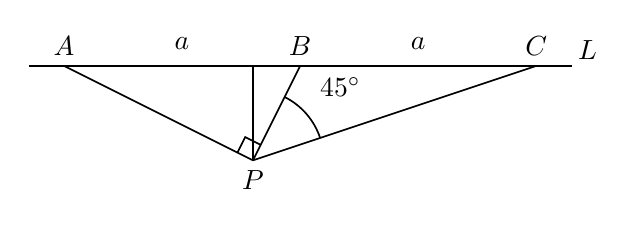
\begin{tikzpicture}[x=1cm,y=1cm,font=\normalsize,line width=.6pt]
\coordinate (A) at (-3.0000,0.0000);
\coordinate (B) at (0.0000,0.0000);
\coordinate (C) at (3.0000,0.0000);
\coordinate (P) at (-0.6000,-1.2000);
\coordinate (H) at (-0.6000,0.0000);
% 直线 L 与线段
\draw (-3.4500,0.0000)--(3.4500,0.0000);
\draw (P)--(A);
\draw (P)--(B);
\draw (P)--(C);
\draw (P)--(H);
% 直角标记 ∠APB = 90°
\draw (-0.5016,-1.0032)--(-0.6984,-0.9048)--(-0.7968,-1.1016);
% ∠BPC = 45°
\draw (P) ++(18.435:0.90) arc[start angle=18.435,end angle=63.435,radius=0.90];
\node at (0.5108,-0.2680) {$45^{\circ}$};
% 点与边长标签
\node[above] at (A) {$A$};
\node[above] at (B) {$B$};
\node[above] at (C) {$C$};
\node at (-1.5000,0.2800) {$a$};
\node at (1.5000,0.2800) {$a$};
\node[below] at (P) {$P$};
\node[anchor=south west,inner sep=0pt,xshift=2pt,yshift=2pt] at (3.45,0) {$L$};
\end{tikzpicture}
